%!TEX root=masterproef.tex

\chapter{Architectuur}
\label{chapter:architectuur}

De oplossingsstrategie stelt voor om een uitwendige DSL te combineren met code
generatie om zo een volledig geautomatiseerde keten te bekomen van onderzoek
tot uitbating. Dit hoofdstuk bekijkt de oplossing vanuit een architectuur
oogpunt.

In sectie \ref{section:arch-functional} overlopen we de functionaliteit van de
oplossing en identificeren de verschillende functionele componenten en de
onderlinge relaties. Dit overzicht identificeert tevens de scope die zal
aangehouden worden in het vervolg van deze thesis.

De functionele architectuur wordt in sectie \ref{section:arch-technical}
uitgewerkt in een technische architectuur. Hier wordt het functionele proces
opgedeeld in technische componenten en worden de verschillende interne
informatiestromen, -manipulaties en -opslagvormen.

\section{Functionele architectuur}
\label{section:arch-functional}

Figuur \ref{fig:arch-functional} geeft een overzicht van de voorgestelde
oplossing.

\begin{figure}[ht]
  \centering
  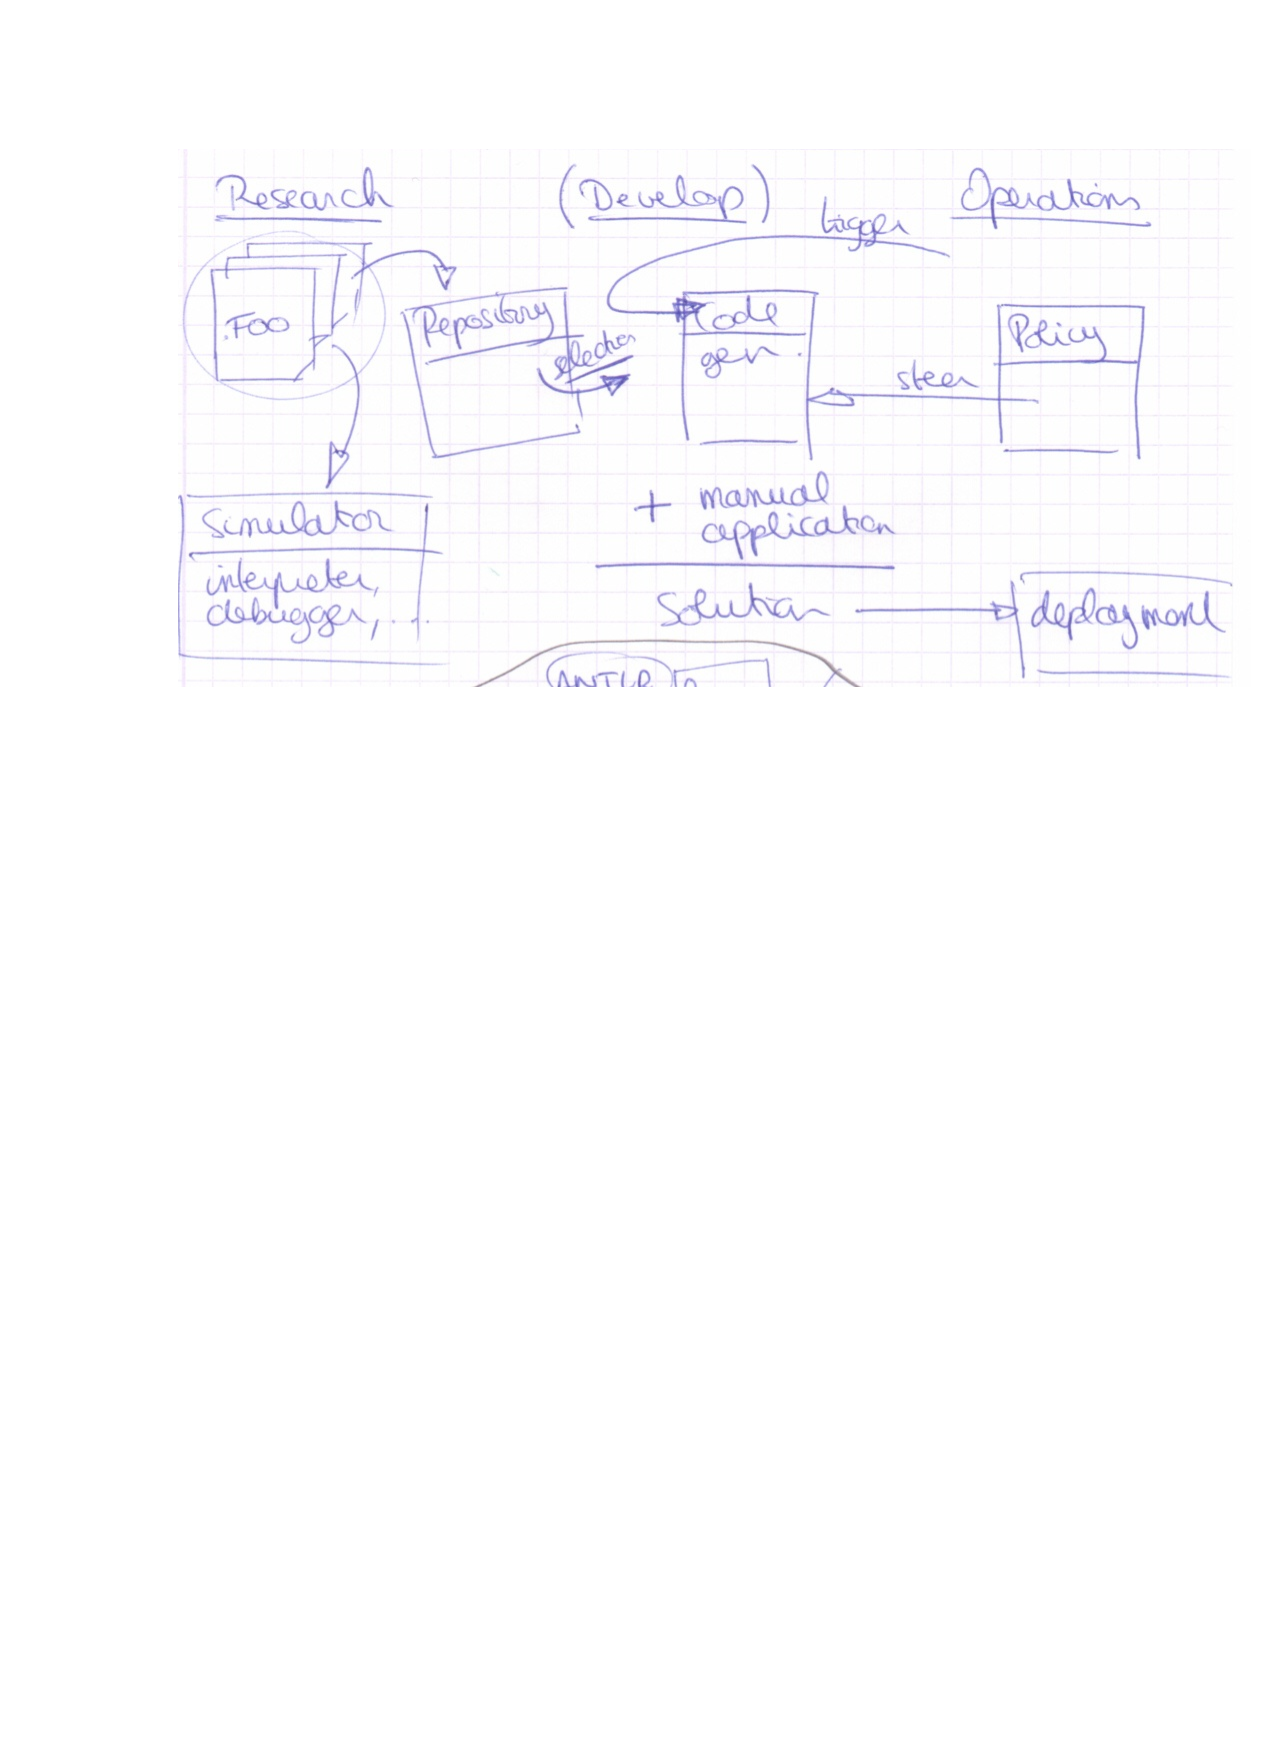
\includegraphics[width=\linewidth]{resources/arch-functional.pdf}
  \caption{Functionele architectuur}
  \label{fig:arch-functional}
\end{figure}

\subsection{FOO-lang}
\label{subsection:arch-foo-lang}

De eerste belangrijke component van de oplossing is de domeinspecifieke taal,
waarmee detectiealgoritmes kunnen beschreven worden. De belangrijkste
doelstelling van de taal is om de functionaliteit zo optimaal mogelijk te
organiseren. Hierdoor wordt getracht om het gebruik van de \mcu en het gebruik
van de draadloze radio te beperken. Deze doelstelling wordt ook weerspiegeld in
de naam: Functie Organisatie Optimalisatie (Engels: Function Organisation
Optimisation), kortweg: FOO-lang.

De belangrijkste doelgroep wat betreft gebruikers, zijn onderzoekers van IDS in
WSN. Met FOO-lang kunnen zij beschikken over een formele taal om
inbraakdetectiealgoritmes voor WSN te beschrijven.

Het is van primordiaal belang dat de taal zo dicht mogelijk aansluit bij
bestaande kennis en vertrouwde paradigma. Daarom wordt voorgesteld om dicht bij
de C programmeertaal aan te blijven leunen en deze uit te breiden met niet
ongewone constructies om het niveau van de taal op een hoger niveau van
abstractie te brengen. Dit hogere niveau sluit meer aan bij een functionele en
platform-onafhankelijke beschrijving.

Om de doelstelling na te streven is het belangrijk dat er control is over de
iteratieve aspecten van de algoritmen. Deze gaan typisch om de sensorknopen in
de nabijheid van de knoop in kwestie. Door de functionaliteit van het domein te
centraliseren rond deze knopen, is het mogelijk om deze iteraties weg te
werken. Door het defini\"eren van gebeurtenissen waarop kan gereageerd worden
met functionaliteit, is het mogelijk om abstractie te maken van de volledige
lijst van sensorknopen en het algoritme in stukken te breken die als reacties
op de gebeurtenissen kunnen beschreven worden.

Om het functionele karakter verder te onderstrepen is het belangrijk dat zoveel
mogelijk technische aspecten uit de algoritmen geweerd worden. Een typische
voorbeeld is de typering van variabelen. Typering zal een noodzaak blijken,
maar moet op zijn minst optioneel zijn en indien nodig voorzien worden als een
beperkte set van functionele types. Dit is ook een belangrijke voorwaarde voor
de platform-onafhankelijkheid.

\subsection{Centrale opslagplaats}
\label{subsection:arch-repository}

\TODO

\subsection{Code generator}
\label{subsection:arch-codegen}

\TODO

\subsection{Uitbatingsbeleid}
\label{subsection:arch-policy}

\TODO

\subsection{Ontwikkeling en integratie}
\label{subsection:arch-integration}

\TODO

\subsection{Scope}
\label{subsection:arch-scope}

\TODO

\section{Technische architectuur}
\label{section:arch-technical}

\TODO

\begin{figure}[ht]
  \centering
  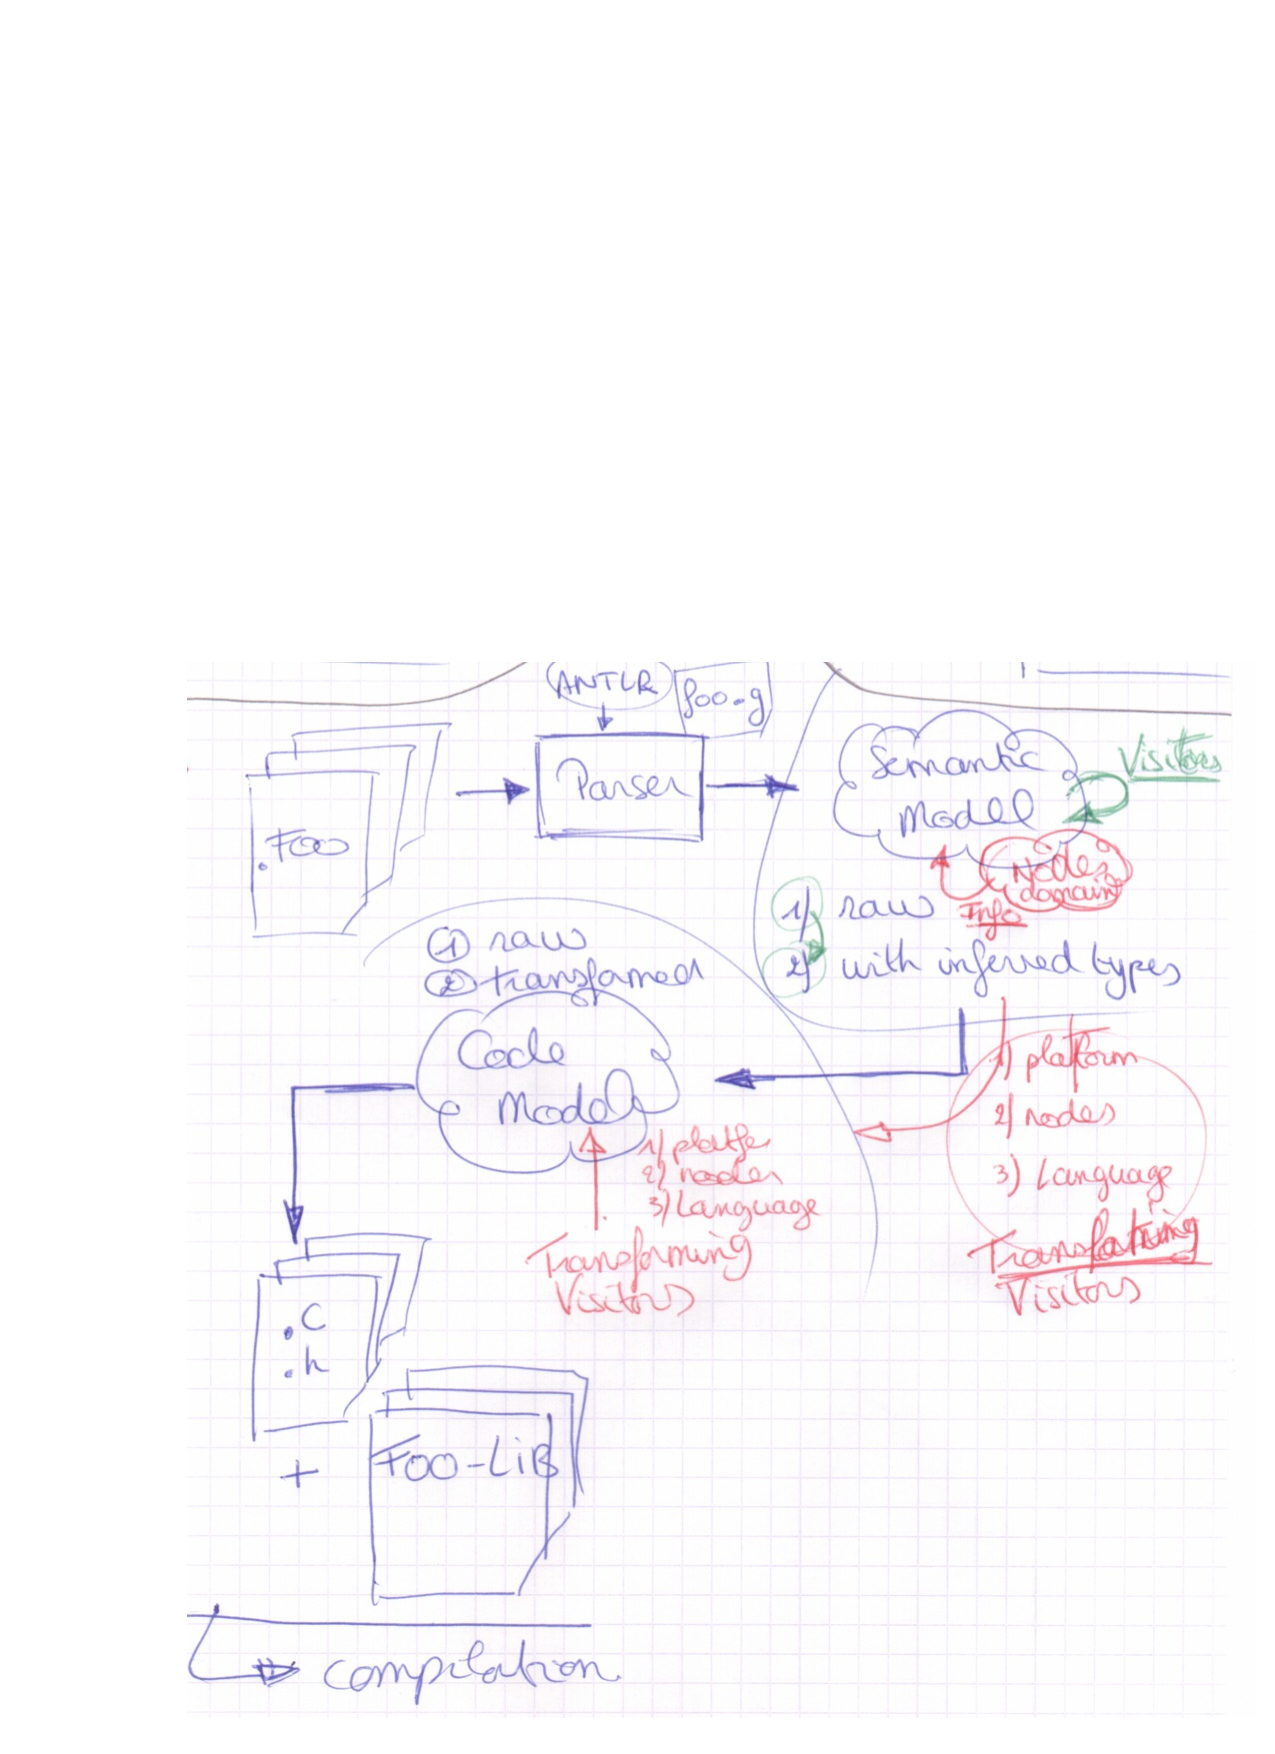
\includegraphics[width=\linewidth]{resources/arch-technical.pdf}
  \caption{Technische architectuur}
  \label{fig:arch-technical}
\end{figure}

\subsection{Semantisch model}
\label{subsection:arch-semantic-model}

\TODO \citep{fowler2010domain}

\subsection{Code model}
\label{subsection:arch-code-model}

\TODO

